\title{Fourier from the ground up}


\section{The algebra of trigonometric polynomials}


\newcommand{\Z}{\mathbf{Z}}
\newcommand{\R}{\mathbf{R}}
\newcommand{\C}{\mathbf{C}}
\newcommand{\PP}{\mathcal{P}}

\begin{definition}
A~\emph{trigonometric polynomial} is an expression of the form
$$
	f(\theta)=\sum_{n\in\Z} f_n e^{in\theta}
$$
where all the coefficients~$f_n\in\C$ are zero except, maybe, a finite
number of them.  The set of all trigonometric polynomials is denoted
by~$\PP$.
\end{definition}

There are two ways to interpret a trigonometric polynomial: as a
function~$\Z\to\C$ defined by~$n\mapsto f_n$, or as a function~$\R\to\C$
defined by~$\theta\mapsto f(\theta)$.  Most of Fourier analysis deals with
the duality between these two interpretations.

Let us introduce some {\bf common language}.
A trigonometric polynomial is usually called a~\emph{signal}.  The
indices~$n$ are called the~\emph{frequencies} and the coefficient~$f_n$
is called the~\emph{amplitude of~$f$~at the frequency~$n$}.  The
mapping~$n\mapsto\left|f_n\right|^2$ is called the~\emph{power
spectrum} of the signal~$f$.  Building the signal from its amplitudes
is called is called~\emph{synthesis}, and extracting the amplitudes
from a signal is called~\emph{analysis}.

The monomial~$e^{in\theta}$ is called a~\emph{pure wave of frequency~$n$}.
Thus, synthesis consists in creating a signal as a linear combination of pure
waves, and analysis consists in recovering the coefficients of this linear
combination.  The whole of harmonic analysis consists in studying the duality
between signals~$f(\theta)$ and their spectra~$f_n$; how do the operations on
signals correspond to operations on their spectra, and vice-versa.

\begin{definition}
	a b c
\end{definition}

%{\bf Proposition (algebraic properties of~$\PP$).}
%The space~$\PP$ is a vector space over~$\C$ and also an algebra.  The
%(algebraic) inner product on~$\PP$
%$$
%\left\langle f,g\right\rangle_a=\sum_{n\in\Z}f_n\bar{g_n}
%$$ is hermitian, and with the associated
%norm~$\|f\|_a=\sqrt{\left\langle f,f\right\rangle_a}$, the set of
%monomials~$e^{in\theta}$ is an orthonormal basis of~$\PP$.
%This vector space is neither finite-dimensional nor complete with this norm.

\begin{proposition}
(Elementary properties)
The following properties hold:
\begin{enumerate}
	\item If~$f\in\PP$ then~$f(\theta)$ is a
		function~$\R\to\C$ which is~$2\pi$-periodic
		and~$\mathcal{C}^\infty$.
	\item If~$f\in\PP$ then~$f_n$ is a function~$\Z\to\C$ of finite
		support.
	\item The set~$\PP$ is a vector space over~$\C$.
	\item If~$h=\lambda f+\mu g$ then~$h_n=\lambda f_n+\mu g_n$.
	\item The set~$\PP$ is an algebra (thus, closed by
		pointwise product~$f(\theta)g(\theta)$)
\end{enumerate}
\end{proposition}

\begin{proof}
(1) Each monomial~$e^{in\theta}$ is~$\mathcal{C}^\infty$
	and~$2\pi$-periodic, and~$f$ is a finite linear
	combination of such monomials, so it is
	also~$\mathcal{C}^\infty$ and~$2\pi$-periodic.
(2) This is a rewriting of the defintion of~$\PP$.
(3,4) This result is immediate by linearity of finite sums.
(5) The product of two finite sums is still a finite sum.
\end{proof}


When interpreting a trigonometric polynomial as a~$2\pi$-periodic
function~$\R\to\C$, it helps to plot it as a closed curve in the complex
plane.  The monomials~$e^{in\theta}$ for~$n\neq 0$ all correspond to the unit
circle traversed~$n$ times, clockwise for~$n<0$, anticlockwise for~$n>0$.

\begin{tabular}{ccccccc}
	$e^{-3i\theta}$ &
	$e^{-2i\theta}$ &
	$e^{-i\theta}$ &
	$e^{0i\theta}$ &
	$e^{i\theta}$ &
	$e^{2i\theta}$ &
	$e^{3i\theta}$ \\
	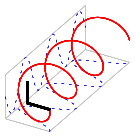
\includegraphics{monomial-3.png} &
	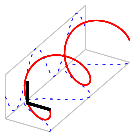
\includegraphics{monomial-2.png} &
	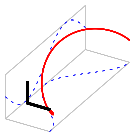
\includegraphics{monomial-1.png} &
	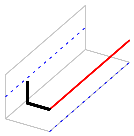
\includegraphics{monomial+0.png} &
	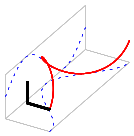
\includegraphics{monomial+1.png} &
	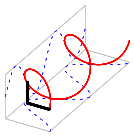
\includegraphics{monomial+2.png} &
	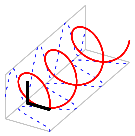
\includegraphics{monomial+3.png} \\
	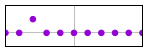
\includegraphics{monoal-3.png} &
	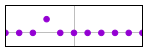
\includegraphics{monoal-2.png} &
	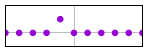
\includegraphics{monoal-1.png} &
	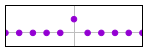
\includegraphics{monoal+0.png} &
	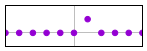
\includegraphics{monoal+1.png} &
	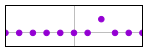
\includegraphics{monoal+2.png} &
	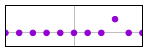
\includegraphics{monoal+3.png} \\
\end{tabular}
%SCRIPT cat <<END >monomial.g
%SCRIPT set term pngcairo crop size 160,160
%SCRIPT unset key; unset border; unset xtics; unset ytics; unset ztics
%SCRIPT set samples 1000; set parametric; set view equal xyz
%SCRIPT set margins at screen 0, at screen 1, at screen 0, at screen 1
%SCRIPT splot [0:2*pi] [-1:1] [-1:1] \
%SCRIPT 	-1,u,-1              lw 0 lc rgb "gray"                  ,\
%SCRIPT 	-1,u,+1              lw 0 lc rgb "gray"                  ,\
%SCRIPT 	+1,u,-1              lw 0 lc rgb "gray"                  ,\
%SCRIPT 	(u-pi)/pi,0,-1       lw 0 lc rgb "gray"                  ,\
%SCRIPT 	(u-pi)/pi,2*pi,-1    lw 0 lc rgb "gray"                  ,\
%%SCRIPT 	(u-pi)/pi,2*pi,+1    lw 0 lc rgb "gray"                  ,\
%SCRIPT 	-1,0,(u-pi)/pi       lw 0 lc rgb "gray"                  ,\
%SCRIPT 	-1,2*pi,(u-pi)/pi    lw 0 lc rgb "gray"                  ,\
%%SCRIPT 	+1,2*pi,(u-pi)/pi    lw 0 lc rgb "gray"                  ,\
%SCRIPT 	cos(f*u),u,-1        lw 0 lc rgb "blue" dashtype '- '    ,\
%SCRIPT 	-1,u,sin(f*u)        lw 0 lc rgb "blue" dashtype '- '    ,\
%%SCRIPT 	cos(f*u),2*pi,sin(f*u) lw 0 lc rgb "blue" dashtype '- '  ,\
%SCRIPT 	cos(f*u),u,sin(f*u)  lw 1 lc rgb "red"                   ,\
%SCRIPT 	u/(2*pi),0,0         lw 2 lc rgb "black"                 ,\
%SCRIPT 	0,0,u/(2*pi)         lw 2 lc rgb "black"
%SCRIPT END
%SCRIPT gnuplot -e "f=+0" monomial.g > monomial+0.png &
%SCRIPT gnuplot -e "f=+1" monomial.g > monomial+1.png &
%SCRIPT gnuplot -e "f=+2" monomial.g > monomial+2.png &
%SCRIPT gnuplot -e "f=+3" monomial.g > monomial+3.png &
%SCRIPT gnuplot -e "f=-1" monomial.g > monomial-1.png &
%SCRIPT gnuplot -e "f=-2" monomial.g > monomial-2.png &
%SCRIPT gnuplot -e "f=-3" monomial.g > monomial-3.png &
%SCRIPT wait

%SCRIPT cat <<END >mz.g
%SCRIPT set term pngcairo crop size 192,192
%SCRIPT unset key;unset xtics; unset ytics; set size ratio -1
%SCRIPT set zeroaxis lw 1 lc rgb "gray" lt 1
%SCRIPT plot [-5:5] [-1:2] "< cat -" w circles fill solid
%SCRIPT END
%SCRIPT X=`seq -5 5`
%SCRIPT for i in $X; do echo $i $((i==-3)); done |gnuplot mz.g >monoal-3.png &
%SCRIPT for i in $X; do echo $i $((i==-2)); done |gnuplot mz.g >monoal-2.png &
%SCRIPT for i in $X; do echo $i $((i==-1)); done |gnuplot mz.g >monoal-1.png &
%SCRIPT for i in $X; do echo $i $((i==+0)); done |gnuplot mz.g >monoal+0.png &
%SCRIPT for i in $X; do echo $i $((i==+1)); done |gnuplot mz.g >monoal+1.png &
%SCRIPT for i in $X; do echo $i $((i==+2)); done |gnuplot mz.g >monoal+2.png &
%SCRIPT for i in $X; do echo $i $((i==+3)); done |gnuplot mz.g >monoal+3.png &
%SCRIPT wait





% vim:set tw=77 filetype=tex spell spelllang=en:
